\documentclass{article}
\usepackage[utf8]{inputenc}

\usepackage{natbib}
\usepackage{graphicx}

% margins well 
\usepackage{geometry}
\geometry{margin=1in}

\usepackage{amsmath} % math symbols

\setlength\parindent{0pt} % No paragraph indents
\newcommand{\forceindent}{\vspace{0em}\leavevmode{\parindent=2em\indent}} % Command to force indent

\usepackage{wrapfig}

\begin{document}
	
	\section{Model}
	
	\begin{wrapfigure}{r}{0.35\textwidth}
		\footnotesize
		\centering
		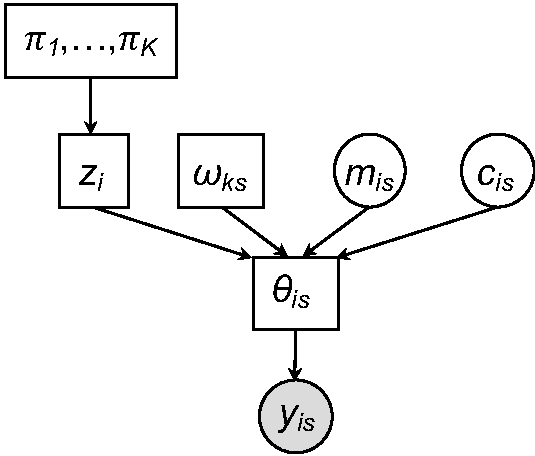
\includegraphics[width=.35\textwidth]{figs/graphical-model-6.pdf}
		\vspace{0em}
		\caption{Bayesian hierarchical model for variant clustering and MCF estimation.}
		\label{fig:model}
	\end{wrapfigure}
	
	
	Indices: 
	\begin{itemize}
		\item Variant $i \in \{1, ..., I\}$
		\item Cluster $k \in \{1, ..., K\}$
		\item Sample $s \in \{1, ..., S\}$
	\end{itemize}
	
	Variables:
	\begin{itemize}
		\item $y[i,s]$ = variant read counts $\sim$ Binomial(n[i,s], $\theta$[i,s])
		\item $n[i,s]$ = total read count (depth)
		\item $m[i,s]$ = multiplicity (\# of variant alleles)
		\item $c[i,s]$ = total copy number 
		
		\item $\omega[k,s] \in (0, 1]$; mutant cell fraction (MCF) \\
		\forceindent prior: Beta(1,1)
		
		\item $z[i] \in \{1, ..., K\}$; cluster membership of variant \\
		\forceindent prior: Categorical($\pi$)
		
		\item $\pi[k] \in (0,1)$; proportion of variants in each cluster \\
		\forceindent prior: Dirichlet(1, ..., 1)
		
		\item $\theta[i,s] \in (0, 1]$; variant allele frequency (VAF) \\
		\forceindent deterministic function of $\omega, m, c, n, z$ \\
		\forceindent $\theta[i,s] = \cfrac{m[i,s] \times \omega[z[i], s]}{c[i,s] \times \omega[z[i], s] + 2\times(1 - \omega[z[i], s])}$
	\end{itemize}
	
	
	\section{Current scheme}
	
	\begin{enumerate}
		\item Split variants into sets based on presence in samples. Each set makes up a "box" in crude tree structure. Ordering of variants is limited by this structure -- can only make vertical connections.
		\item Within each box, cluster variants and estimate MCFs. Use BIC to determine number of clusters, k. 
		\item Order variant clusters (i.e. connect cluster nodes to form tree). 
	\end{enumerate}
	
	\section{Problems/Issues}
	
	\begin{itemize}
		\item P(tree $|$ data) ?
		\item Clustering and CCF estimation is done within a box, but tree spans all boxes 
		
		
	\end{itemize}
	
	%\bibliographystyle{plain}
	%\bibliography{references}
\end{document}
